\section{Sujetos}
El presente proyecto se trabaj\'o en el departamento de Deportes del campus central de la universidad Rafael Land\'ivar, en las instalaciones del Polideportivo 1. As\'i mismo la unidad de Deportes proporcion\'o trabajar con tres equipos deportivos:
\begin{itemize}
	\item \textbf{Tenis de mesa:} Deporte de raqueta que se juega sobre una mesa rectangular de manera individual o en parejas, con el fin objetivo de golpear una peque\~na pelota.
	\item \textbf{Animaci\'on:} Deporte grupal que combina la m\'usica y gimnasia, a partir de rutinas de baile que entusiasma un p\'ublico o evento deportivo.
	\item \textbf{Taekwondo:} Deporte individual basado en el arte marcial coreano moderno, que consiste en el uso de los p\'ies, brazos y pu\~nos dentro de un combate.
\end{itemize}
\subsection{Primer tipo} \label{sj:1t}
Define la cantidad de sujetos que participaron en la recolecta de los datos para la creaci\'on del modelo de reconocimiento del movimiento, a partir de tres fases distintas:
\begin{itemize}
	\item \textbf{Construci\'on:} Atletas que construyeron el modelo continuo de machine learning.
	\item \textbf{Pruebas:} Muestra de usuarios que se emple\'o para el c\'alculo de los errores de pron\'ostico del modelo.
	\item \textbf{Validaci\'on:} Conjunto de deportistas que realizaron pruebas al modelo, en tiempo real.
\end{itemize}
\subsubsection{Equipo de animaci\'on de la universidad rafael land\'ivar} \label{sj:1t:ani}
\begin{table}[H]
\begin{center}
\caption{Muestra del equipo de animadoras}
\label{tab:MuestraCheerleaders}
\begin{tabular}{lc}
\hline
\multicolumn{1}{|l|}{\textbf{Descripci\'on}} & \multicolumn{1}{l|}{\textbf{Cantidad}} \\ \hline
\multicolumn{1}{|l|}{Atletas para la construci\'on del modelo} & \multicolumn{1}{c|}{6} \\ \hline
\multicolumn{1}{|l|}{Atletas para la pruebas del modelo} & \multicolumn{1}{c|}{1} \\ \hline
\multicolumn{1}{|l|}{Atletas para la validaci\'on del modelo} & \multicolumn{1}{c|}{2} \\ \hline
\multicolumn{1}{|r|}{Total de atletas} & \multicolumn{1}{c|}{9} \\ \hline
\textbf{Fuente:} Observaci\'on del investigador durante el trabajo de campo.
\end{tabular}
\end{center}
\end{table}
\subsubsection{Equipo de tenis de mesa de la universidad rafael land\'ivar}\label{sj:1t:ten}
\begin{table}[H]
\begin{center}
\caption{Muestra del equipo de tenis de mesa}
\label{tab:MuestraTenis}
\begin{tabular}{lc}
\hline
\multicolumn{1}{|l|}{\textbf{Descripci\'on}} & \multicolumn{1}{l|}{\textbf{Cantidad}} \\ \hline
\multicolumn{1}{|l|}{Atletas para la construci\'on del modelo} & \multicolumn{1}{c|}{5} \\ \hline
\multicolumn{1}{|l|}{Atletas para la pruebas del modelo} & \multicolumn{1}{c|}{1} \\ \hline
\multicolumn{1}{|l|}{Atletas para la validaci\'on del modelo} & \multicolumn{1}{c|}{3} \\ \hline
\multicolumn{1}{|r|}{Total de atletas} & \multicolumn{1}{c|}{9} \\ \hline
\textbf{Fuente:} Observaci\'on del investigador durante el trabajo de campo.
\end{tabular}
\end{center}
\end{table}
\subsubsection{Equipo de taekwondo de la universidad rafael land\'ivar}\label{sj:1t:tae}
\begin{table}[H]
\begin{center}
\caption{Muestra del equipo de taekwondo}
\label{tab:MuestraTaekwondo}
\begin{tabular}{lc}
\hline
\multicolumn{1}{|l|}{\textbf{Descripci\'on}} & \multicolumn{1}{l|}{\textbf{Cantidad}} \\ \hline
\multicolumn{1}{|l|}{Atletas para la construci\'on del modelo} & \multicolumn{1}{c|}{13} \\ \hline
\multicolumn{1}{|l|}{Atletas para la pruebas del modelo} & \multicolumn{1}{c|}{1} \\ \hline
\multicolumn{1}{|r|}{Total de atletas} & \multicolumn{1}{c|}{14} \\ \hline
\textbf{Fuente:} Observaci\'on del investigador durante el trabajo de campo.
\end{tabular}
\end{center}
\end{table}
\subsection{Segundo tipo} \label{sj:2t}
A continuaci\'on se muestra un organigrama de la estructura del departamento de deportes de la universidad Rafael Land\'ivar, en ella se muestra todos los profesionales que aportaron en la investigaci\'on:
\begin{figure}[H]
	\caption{Organigrama del departamentos de deportes de la Universidad Rafael Land\'ivar}
	\label{fig:orgDeportes}
	\centering
	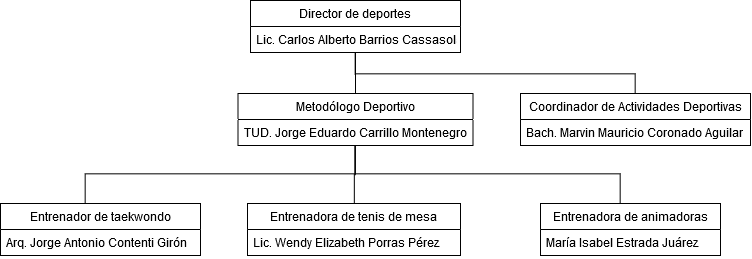
\includegraphics[width=450px,height=170px]{graphics/orgDeportes.png} \\
	\textbf{Fuente:} Elaborado por el autor de tesis
\end{figure}
\subsection{Unidades de an\'alisis} \label{sj:ua}
Para el presente proyecto se utiliz\'o como referencia el manual de acondicionamiento de fuerza y prevensi\'on de lesiones  \cite{arbour2006strength}, la cual describe los movimientos ideales para el calentamiento  y estiramiento de una rutina -i.e. Warm up- (Ver secci\'on de anexos \ref{anx:warmup}).